% Options for packages loaded elsewhere
\PassOptionsToPackage{unicode}{hyperref}
\PassOptionsToPackage{hyphens}{url}
%
\documentclass[
]{article}
\usepackage{amsmath,amssymb}
\usepackage{lmodern}
\usepackage{iftex}
\ifPDFTeX
  \usepackage[T1]{fontenc}
  \usepackage[utf8]{inputenc}
  \usepackage{textcomp} % provide euro and other symbols
\else % if luatex or xetex
  \usepackage{unicode-math}
  \defaultfontfeatures{Scale=MatchLowercase}
  \defaultfontfeatures[\rmfamily]{Ligatures=TeX,Scale=1}
\fi
% Use upquote if available, for straight quotes in verbatim environments
\IfFileExists{upquote.sty}{\usepackage{upquote}}{}
\IfFileExists{microtype.sty}{% use microtype if available
  \usepackage[]{microtype}
  \UseMicrotypeSet[protrusion]{basicmath} % disable protrusion for tt fonts
}{}
\makeatletter
\@ifundefined{KOMAClassName}{% if non-KOMA class
  \IfFileExists{parskip.sty}{%
    \usepackage{parskip}
  }{% else
    \setlength{\parindent}{0pt}
    \setlength{\parskip}{6pt plus 2pt minus 1pt}}
}{% if KOMA class
  \KOMAoptions{parskip=half}}
\makeatother
\usepackage{xcolor}
\IfFileExists{xurl.sty}{\usepackage{xurl}}{} % add URL line breaks if available
\IfFileExists{bookmark.sty}{\usepackage{bookmark}}{\usepackage{hyperref}}
\hypersetup{
  pdftitle={exam},
  pdfauthor={202121225 통계학과 서하진},
  hidelinks,
  pdfcreator={LaTeX via pandoc}}
\urlstyle{same} % disable monospaced font for URLs
\usepackage[margin=1in]{geometry}
\usepackage{color}
\usepackage{fancyvrb}
\newcommand{\VerbBar}{|}
\newcommand{\VERB}{\Verb[commandchars=\\\{\}]}
\DefineVerbatimEnvironment{Highlighting}{Verbatim}{commandchars=\\\{\}}
% Add ',fontsize=\small' for more characters per line
\usepackage{framed}
\definecolor{shadecolor}{RGB}{248,248,248}
\newenvironment{Shaded}{\begin{snugshade}}{\end{snugshade}}
\newcommand{\AlertTok}[1]{\textcolor[rgb]{0.94,0.16,0.16}{#1}}
\newcommand{\AnnotationTok}[1]{\textcolor[rgb]{0.56,0.35,0.01}{\textbf{\textit{#1}}}}
\newcommand{\AttributeTok}[1]{\textcolor[rgb]{0.77,0.63,0.00}{#1}}
\newcommand{\BaseNTok}[1]{\textcolor[rgb]{0.00,0.00,0.81}{#1}}
\newcommand{\BuiltInTok}[1]{#1}
\newcommand{\CharTok}[1]{\textcolor[rgb]{0.31,0.60,0.02}{#1}}
\newcommand{\CommentTok}[1]{\textcolor[rgb]{0.56,0.35,0.01}{\textit{#1}}}
\newcommand{\CommentVarTok}[1]{\textcolor[rgb]{0.56,0.35,0.01}{\textbf{\textit{#1}}}}
\newcommand{\ConstantTok}[1]{\textcolor[rgb]{0.00,0.00,0.00}{#1}}
\newcommand{\ControlFlowTok}[1]{\textcolor[rgb]{0.13,0.29,0.53}{\textbf{#1}}}
\newcommand{\DataTypeTok}[1]{\textcolor[rgb]{0.13,0.29,0.53}{#1}}
\newcommand{\DecValTok}[1]{\textcolor[rgb]{0.00,0.00,0.81}{#1}}
\newcommand{\DocumentationTok}[1]{\textcolor[rgb]{0.56,0.35,0.01}{\textbf{\textit{#1}}}}
\newcommand{\ErrorTok}[1]{\textcolor[rgb]{0.64,0.00,0.00}{\textbf{#1}}}
\newcommand{\ExtensionTok}[1]{#1}
\newcommand{\FloatTok}[1]{\textcolor[rgb]{0.00,0.00,0.81}{#1}}
\newcommand{\FunctionTok}[1]{\textcolor[rgb]{0.00,0.00,0.00}{#1}}
\newcommand{\ImportTok}[1]{#1}
\newcommand{\InformationTok}[1]{\textcolor[rgb]{0.56,0.35,0.01}{\textbf{\textit{#1}}}}
\newcommand{\KeywordTok}[1]{\textcolor[rgb]{0.13,0.29,0.53}{\textbf{#1}}}
\newcommand{\NormalTok}[1]{#1}
\newcommand{\OperatorTok}[1]{\textcolor[rgb]{0.81,0.36,0.00}{\textbf{#1}}}
\newcommand{\OtherTok}[1]{\textcolor[rgb]{0.56,0.35,0.01}{#1}}
\newcommand{\PreprocessorTok}[1]{\textcolor[rgb]{0.56,0.35,0.01}{\textit{#1}}}
\newcommand{\RegionMarkerTok}[1]{#1}
\newcommand{\SpecialCharTok}[1]{\textcolor[rgb]{0.00,0.00,0.00}{#1}}
\newcommand{\SpecialStringTok}[1]{\textcolor[rgb]{0.31,0.60,0.02}{#1}}
\newcommand{\StringTok}[1]{\textcolor[rgb]{0.31,0.60,0.02}{#1}}
\newcommand{\VariableTok}[1]{\textcolor[rgb]{0.00,0.00,0.00}{#1}}
\newcommand{\VerbatimStringTok}[1]{\textcolor[rgb]{0.31,0.60,0.02}{#1}}
\newcommand{\WarningTok}[1]{\textcolor[rgb]{0.56,0.35,0.01}{\textbf{\textit{#1}}}}
\usepackage{graphicx}
\makeatletter
\def\maxwidth{\ifdim\Gin@nat@width>\linewidth\linewidth\else\Gin@nat@width\fi}
\def\maxheight{\ifdim\Gin@nat@height>\textheight\textheight\else\Gin@nat@height\fi}
\makeatother
% Scale images if necessary, so that they will not overflow the page
% margins by default, and it is still possible to overwrite the defaults
% using explicit options in \includegraphics[width, height, ...]{}
\setkeys{Gin}{width=\maxwidth,height=\maxheight,keepaspectratio}
% Set default figure placement to htbp
\makeatletter
\def\fps@figure{htbp}
\makeatother
\setlength{\emergencystretch}{3em} % prevent overfull lines
\providecommand{\tightlist}{%
  \setlength{\itemsep}{0pt}\setlength{\parskip}{0pt}}
\setcounter{secnumdepth}{-\maxdimen} % remove section numbering
\ifLuaTeX
  \usepackage{selnolig}  % disable illegal ligatures
\fi

\title{exam}
\author{202121225 통계학과 서하진}
\date{12/21/2021}

\begin{document}
\maketitle

\#\#\#1-1

\begin{Shaded}
\begin{Highlighting}[]
\NormalTok{i}\OtherTok{\textless{}{-}}\DecValTok{1}\SpecialCharTok{:}\DecValTok{1000}


\NormalTok{epsilon\_i}\OtherTok{\textless{}{-}}\FunctionTok{rnorm}\NormalTok{(}\AttributeTok{n=}\DecValTok{1000}\NormalTok{,}\AttributeTok{mean=}\DecValTok{0}\NormalTok{,}\AttributeTok{sd=}\DecValTok{1}\NormalTok{)}
\end{Highlighting}
\end{Shaded}

\#\#\#1-2

\begin{Shaded}
\begin{Highlighting}[]
\NormalTok{i}\OtherTok{\textless{}{-}}\DecValTok{1}\SpecialCharTok{:}\DecValTok{1000}
\NormalTok{t\_i}\OtherTok{\textless{}{-}}\NormalTok{ \{}\DecValTok{2}\SpecialCharTok{*}\NormalTok{pi}\SpecialCharTok{*}\NormalTok{i\}}\SpecialCharTok{/}\NormalTok{\{}\DecValTok{1000}\NormalTok{\}}
\NormalTok{x1}\OtherTok{\textless{}{-}} \FunctionTok{sin}\NormalTok{(t\_i)}
\NormalTok{x2}\OtherTok{\textless{}{-}} \FunctionTok{cos}\NormalTok{(}\DecValTok{4}\SpecialCharTok{*}\NormalTok{t\_i)}
\end{Highlighting}
\end{Shaded}

\#\#\#1-3

\begin{Shaded}
\begin{Highlighting}[]
\NormalTok{i}\OtherTok{\textless{}{-}}\DecValTok{1}\SpecialCharTok{:}\DecValTok{1000}

\NormalTok{t\_i}\OtherTok{\textless{}{-}}\NormalTok{ \{}\DecValTok{2}\SpecialCharTok{*}\NormalTok{pi}\SpecialCharTok{*}\NormalTok{i\}}\SpecialCharTok{/}\NormalTok{\{}\DecValTok{1000}\NormalTok{\}}

\NormalTok{x1}\OtherTok{\textless{}{-}} \FunctionTok{sin}\NormalTok{(t\_i)}
\NormalTok{x2}\OtherTok{\textless{}{-}} \FunctionTok{cos}\NormalTok{(}\DecValTok{4}\SpecialCharTok{*}\NormalTok{t\_i)}

\NormalTok{y\_i}\OtherTok{\textless{}{-}} \FloatTok{1.5} \SpecialCharTok{+} \DecValTok{5}\SpecialCharTok{*}\NormalTok{x1 }\SpecialCharTok{+} \DecValTok{3}\SpecialCharTok{*}\NormalTok{x2 }\SpecialCharTok{+}\NormalTok{ epsilon\_i}

\FunctionTok{plot}\NormalTok{(t\_i, y\_i, }\AttributeTok{col=}\StringTok{\textquotesingle{}gray60\textquotesingle{}}\NormalTok{)}
\end{Highlighting}
\end{Shaded}

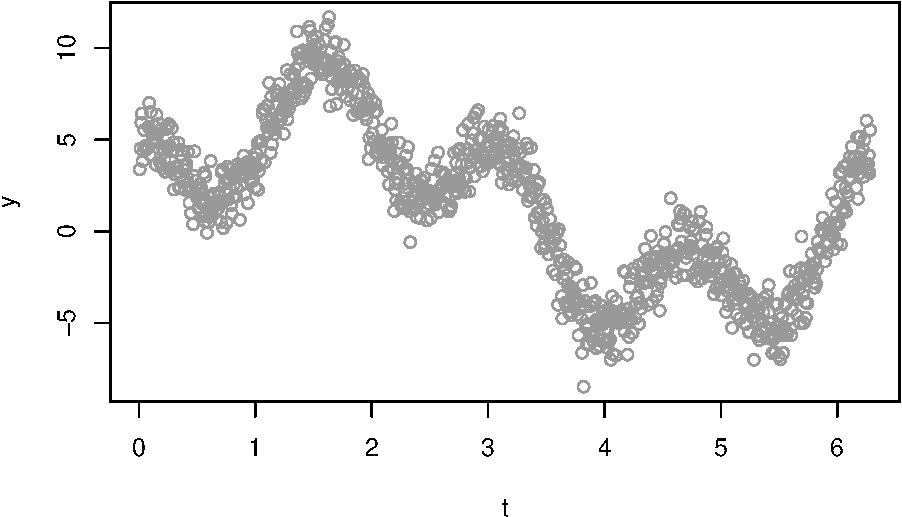
\includegraphics{서하진_exam_pdf_files/figure-latex/unnamed-chunk-3-1.pdf}

\#\#\#1-4

\begin{Shaded}
\begin{Highlighting}[]
\NormalTok{i}\OtherTok{\textless{}{-}}\DecValTok{1}\SpecialCharTok{:}\DecValTok{1000}

\NormalTok{t\_i}\OtherTok{\textless{}{-}}\NormalTok{ \{}\DecValTok{2}\SpecialCharTok{*}\NormalTok{pi}\SpecialCharTok{*}\NormalTok{i\}}\SpecialCharTok{/}\NormalTok{\{}\DecValTok{1000}\NormalTok{\}}

\NormalTok{x1}\OtherTok{\textless{}{-}} \FunctionTok{sin}\NormalTok{(t\_i)}
\NormalTok{x2}\OtherTok{\textless{}{-}} \FunctionTok{cos}\NormalTok{(}\DecValTok{4}\SpecialCharTok{*}\NormalTok{t\_i)}

\NormalTok{X}\OtherTok{=}\FunctionTok{cbind}\NormalTok{(}\DecValTok{1}\NormalTok{,x1,x2)}
\end{Highlighting}
\end{Shaded}

\#\#\#1-5

\begin{Shaded}
\begin{Highlighting}[]
\NormalTok{𝜷}\OtherTok{=}\FunctionTok{cbind}\NormalTok{(}\FunctionTok{c}\NormalTok{(}\FloatTok{1.5}\NormalTok{,}\DecValTok{5}\NormalTok{,}\DecValTok{3}\NormalTok{))}
\NormalTok{X𝜷 }\OtherTok{\textless{}{-}}\NormalTok{ X}\SpecialCharTok{\%*\%}\NormalTok{𝜷}

\FunctionTok{plot}\NormalTok{(t\_i, y\_i, }\AttributeTok{col=}\StringTok{\textquotesingle{}gray60\textquotesingle{}}\NormalTok{)}
\FunctionTok{lines}\NormalTok{(t\_i,X𝜷 , }\AttributeTok{col=}\StringTok{"red"}\NormalTok{,}\AttributeTok{lwd=}\StringTok{\textquotesingle{}5\textquotesingle{}}\NormalTok{)}
\end{Highlighting}
\end{Shaded}

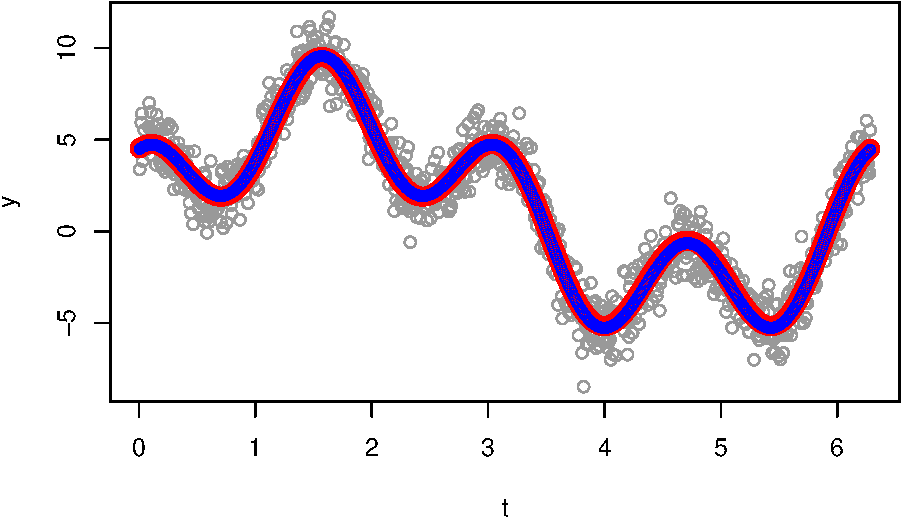
\includegraphics{서하진_exam_pdf_files/figure-latex/unnamed-chunk-5-1.pdf}

\#\#\#1-6

\begin{Shaded}
\begin{Highlighting}[]
\NormalTok{X\_t}\OtherTok{\textless{}{-}}\FunctionTok{t}\NormalTok{(X)}
\NormalTok{XtX\_ }\OtherTok{\textless{}{-}} \FunctionTok{solve}\NormalTok{(X\_t}\SpecialCharTok{\%*\%}\NormalTok{X)}

\NormalTok{hat𝜷}\OtherTok{=}\NormalTok{ XtX\_}\SpecialCharTok{\%*\%}\NormalTok{X\_t}\SpecialCharTok{\%*\%}\NormalTok{y\_i}
\NormalTok{hat𝜷}
\end{Highlighting}
\end{Shaded}

\begin{verbatim}
##        [,1]
##    1.455935
## x1 4.970925
## x2 2.980366
\end{verbatim}

\#\#\#1-7

\begin{Shaded}
\begin{Highlighting}[]
\NormalTok{X\_hat𝜷}\OtherTok{\textless{}{-}}\NormalTok{ X}\SpecialCharTok{\%*\%}\NormalTok{hat𝜷}

\FunctionTok{plot}\NormalTok{(t\_i, y\_i, }\AttributeTok{col=}\StringTok{\textquotesingle{}gray60\textquotesingle{}}\NormalTok{)}
\FunctionTok{lines}\NormalTok{(t\_i,X𝜷 , }\AttributeTok{col=}\StringTok{"red"}\NormalTok{,}\AttributeTok{lwd=}\StringTok{\textquotesingle{}5\textquotesingle{}}\NormalTok{)}
\FunctionTok{lines}\NormalTok{(t\_i,X\_hat𝜷 , }\AttributeTok{lty=}\StringTok{"dashed"}\NormalTok{, }\AttributeTok{col=}\StringTok{"blue"}\NormalTok{,}\AttributeTok{lwd=}\StringTok{\textquotesingle{}5\textquotesingle{}}\NormalTok{)}
\end{Highlighting}
\end{Shaded}

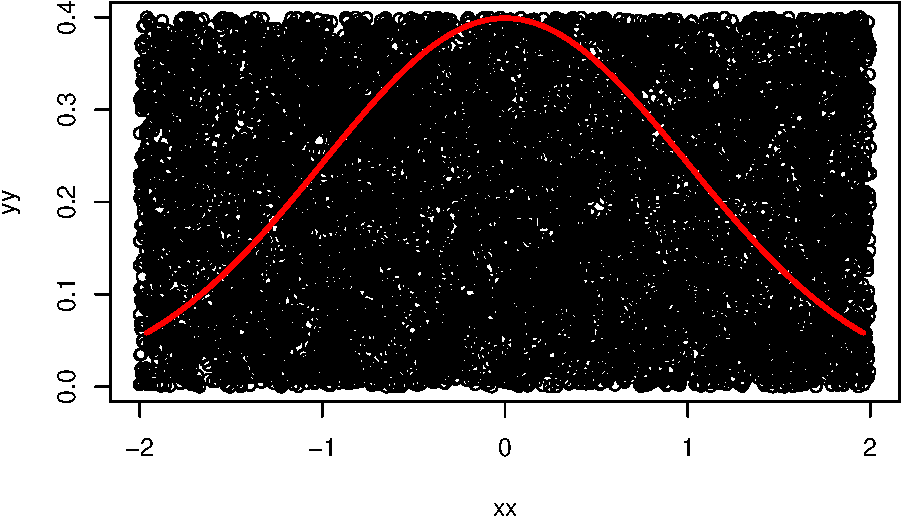
\includegraphics{서하진_exam_pdf_files/figure-latex/unnamed-chunk-7-1.pdf}

\#\#\#2-1

\begin{Shaded}
\begin{Highlighting}[]
\NormalTok{x}\OtherTok{=}\FunctionTok{seq}\NormalTok{(}\AttributeTok{from=}\SpecialCharTok{{-}}\FloatTok{1.96}\NormalTok{,}\AttributeTok{to=}\FloatTok{1.96}\NormalTok{,}\AttributeTok{by=}\FloatTok{0.01}\NormalTok{)}
\NormalTok{y}\OtherTok{=}\NormalTok{(}\DecValTok{1}\SpecialCharTok{/}\FunctionTok{sqrt}\NormalTok{(}\DecValTok{2}\SpecialCharTok{*}\NormalTok{pi))}\SpecialCharTok{*}\FunctionTok{exp}\NormalTok{(}\SpecialCharTok{{-}}\NormalTok{x}\SpecialCharTok{\^{}}\DecValTok{2}\SpecialCharTok{/}\DecValTok{2}\NormalTok{)}

\NormalTok{xx}\OtherTok{=}\FunctionTok{runif}\NormalTok{(}\DecValTok{10000}\NormalTok{)}\SpecialCharTok{*}\DecValTok{4{-}2}
\NormalTok{yy}\OtherTok{=}\FunctionTok{runif}\NormalTok{(}\DecValTok{10000}\NormalTok{)}
\FunctionTok{plot}\NormalTok{(xx,yy)}
\FunctionTok{lines}\NormalTok{(x,y,}\AttributeTok{col=}\StringTok{\textquotesingle{}red\textquotesingle{}}\NormalTok{,}\AttributeTok{lwd=}\DecValTok{3}\NormalTok{)}
\end{Highlighting}
\end{Shaded}

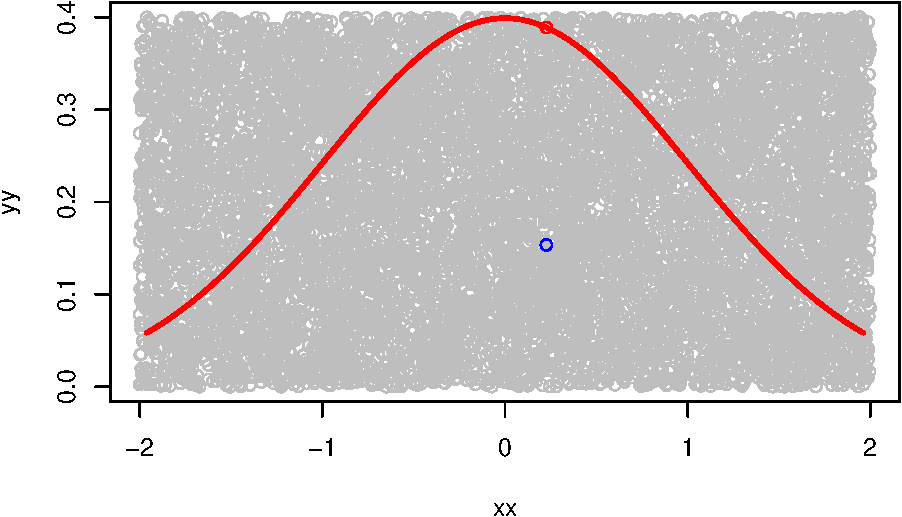
\includegraphics{서하진_exam_pdf_files/figure-latex/unnamed-chunk-8-1.pdf}

\begin{Shaded}
\begin{Highlighting}[]
\NormalTok{test }\OtherTok{=} \ControlFlowTok{function}\NormalTok{(xx,yy)\{}
\NormalTok{    yy }\SpecialCharTok{\textless{}}\NormalTok{ (}\DecValTok{1}\SpecialCharTok{/}\FunctionTok{sqrt}\NormalTok{(}\DecValTok{2}\SpecialCharTok{*}\NormalTok{pi))}\SpecialCharTok{*}\FunctionTok{exp}\NormalTok{(}\SpecialCharTok{{-}}\NormalTok{xx}\SpecialCharTok{\^{}}\DecValTok{2}\SpecialCharTok{/}\DecValTok{2}\NormalTok{)}
\NormalTok{\}}

\FunctionTok{print}\NormalTok{(}\FunctionTok{c}\NormalTok{(xx[}\DecValTok{1}\NormalTok{],yy[}\DecValTok{1}\NormalTok{])) }
\end{Highlighting}
\end{Shaded}

\begin{verbatim}
## [1] -0.4701128  0.4827818
\end{verbatim}

\begin{Shaded}
\begin{Highlighting}[]
\FunctionTok{print}\NormalTok{((}\DecValTok{1}\SpecialCharTok{/}\FunctionTok{sqrt}\NormalTok{(}\DecValTok{2}\SpecialCharTok{*}\NormalTok{pi))}\SpecialCharTok{*}\FunctionTok{exp}\NormalTok{(}\SpecialCharTok{{-}}\NormalTok{xx[}\DecValTok{1}\NormalTok{]}\SpecialCharTok{\^{}}\DecValTok{2}\SpecialCharTok{/}\DecValTok{2}\NormalTok{))}
\end{Highlighting}
\end{Shaded}

\begin{verbatim}
## [1] 0.3572064
\end{verbatim}

\begin{Shaded}
\begin{Highlighting}[]
\FunctionTok{test}\NormalTok{(xx[}\DecValTok{1}\NormalTok{],yy[}\DecValTok{1}\NormalTok{])}
\end{Highlighting}
\end{Shaded}

\begin{verbatim}
## [1] FALSE
\end{verbatim}

\begin{Shaded}
\begin{Highlighting}[]
\FunctionTok{plot}\NormalTok{(xx,yy,}\AttributeTok{col=}\StringTok{\textquotesingle{}gray\textquotesingle{}}\NormalTok{)}
\FunctionTok{lines}\NormalTok{(x,y,}\AttributeTok{col=}\StringTok{\textquotesingle{}red\textquotesingle{}}\NormalTok{,}\AttributeTok{lwd=}\DecValTok{3}\NormalTok{)}
\FunctionTok{points}\NormalTok{(xx[}\DecValTok{1}\NormalTok{],yy[}\DecValTok{1}\NormalTok{],}\AttributeTok{col=}\StringTok{\textquotesingle{}blue\textquotesingle{}}\NormalTok{)}
\FunctionTok{points}\NormalTok{(xx[}\DecValTok{1}\NormalTok{],(}\DecValTok{1}\SpecialCharTok{/}\FunctionTok{sqrt}\NormalTok{(}\DecValTok{2}\SpecialCharTok{*}\NormalTok{pi))}\SpecialCharTok{*}\FunctionTok{exp}\NormalTok{(}\SpecialCharTok{{-}}\NormalTok{xx[}\DecValTok{1}\NormalTok{]}\SpecialCharTok{\^{}}\DecValTok{2}\SpecialCharTok{/}\DecValTok{2}\NormalTok{),}\AttributeTok{col=}\StringTok{\textquotesingle{}red\textquotesingle{}}\NormalTok{)}
\end{Highlighting}
\end{Shaded}

\includegraphics{서하진_exam_pdf_files/figure-latex/unnamed-chunk-8-2.pdf}

\begin{Shaded}
\begin{Highlighting}[]
\NormalTok{tst }\OtherTok{=} \FunctionTok{c}\NormalTok{()}
\ControlFlowTok{for}\NormalTok{ (i }\ControlFlowTok{in} \DecValTok{1}\SpecialCharTok{:}\DecValTok{10000}\NormalTok{) tst[i] }\OtherTok{=} \FunctionTok{test}\NormalTok{(xx[i],yy[i])}
\FunctionTok{head}\NormalTok{(tst)}
\end{Highlighting}
\end{Shaded}

\begin{verbatim}
## [1] FALSE FALSE FALSE FALSE FALSE  TRUE
\end{verbatim}

\begin{Shaded}
\begin{Highlighting}[]
\FunctionTok{plot}\NormalTok{(xx,yy,}\AttributeTok{col=}\StringTok{\textquotesingle{}gray\textquotesingle{}}\NormalTok{)}
\FunctionTok{lines}\NormalTok{(x,y,}\AttributeTok{col=}\StringTok{\textquotesingle{}red\textquotesingle{}}\NormalTok{,}\AttributeTok{lwd=}\DecValTok{3}\NormalTok{)}
\FunctionTok{points}\NormalTok{(xx[tst],yy[tst],}\AttributeTok{col=}\StringTok{\textquotesingle{}red\textquotesingle{}}\NormalTok{)}
\end{Highlighting}
\end{Shaded}

\includegraphics{서하진_exam_pdf_files/figure-latex/unnamed-chunk-8-3.pdf}

\begin{Shaded}
\begin{Highlighting}[]
\FunctionTok{sum}\NormalTok{(tst)}\SpecialCharTok{/}\DecValTok{10000}\SpecialCharTok{*}\DecValTok{4}
\end{Highlighting}
\end{Shaded}

\begin{verbatim}
## [1] 0.9952
\end{verbatim}

\#\#\#2-2

\begin{Shaded}
\begin{Highlighting}[]
\FunctionTok{library}\NormalTok{(tidyverse)}
\end{Highlighting}
\end{Shaded}

\begin{verbatim}
## -- Attaching packages --------------------------------------- tidyverse 1.3.1 --
\end{verbatim}

\begin{verbatim}
## v ggplot2 3.3.5     v purrr   0.3.4
## v tibble  3.1.3     v dplyr   1.0.7
## v tidyr   1.1.3     v stringr 1.4.0
## v readr   1.4.0     v forcats 0.5.1
\end{verbatim}

\begin{verbatim}
## Warning: package 'ggplot2' was built under R version 4.0.5
\end{verbatim}

\begin{verbatim}
## Warning: package 'tibble' was built under R version 4.0.5
\end{verbatim}

\begin{verbatim}
## Warning: package 'tidyr' was built under R version 4.0.3
\end{verbatim}

\begin{verbatim}
## Warning: package 'readr' was built under R version 4.0.5
\end{verbatim}

\begin{verbatim}
## Warning: package 'purrr' was built under R version 4.0.3
\end{verbatim}

\begin{verbatim}
## Warning: package 'dplyr' was built under R version 4.0.5
\end{verbatim}

\begin{verbatim}
## Warning: package 'stringr' was built under R version 4.0.5
\end{verbatim}

\begin{verbatim}
## Warning: package 'forcats' was built under R version 4.0.3
\end{verbatim}

\begin{verbatim}
## -- Conflicts ------------------------------------------ tidyverse_conflicts() --
## x dplyr::filter() masks stats::filter()
## x dplyr::lag()    masks stats::lag()
\end{verbatim}

\begin{Shaded}
\begin{Highlighting}[]
\NormalTok{x}\OtherTok{\textless{}{-}}\FunctionTok{rnorm}\NormalTok{(}\DecValTok{1000}\NormalTok{)}
\FunctionTok{dim}\NormalTok{(x)}\OtherTok{=}\FunctionTok{c}\NormalTok{(}\DecValTok{1000}\NormalTok{,}\DecValTok{1}\NormalTok{)}
\NormalTok{x}\OtherTok{=} \FunctionTok{as\_tibble}\NormalTok{(x)}
\end{Highlighting}
\end{Shaded}

\begin{verbatim}
## Warning: The `x` argument of `as_tibble.matrix()` must have unique column names if `.name_repair` is omitted as of tibble 2.0.0.
## Using compatibility `.name_repair`.
## This warning is displayed once every 8 hours.
## Call `lifecycle::last_lifecycle_warnings()` to see where this warning was generated.
\end{verbatim}

\begin{Shaded}
\begin{Highlighting}[]
\NormalTok{x }\SpecialCharTok{\%\textgreater{}\%} \FunctionTok{filter}\NormalTok{(V1}\SpecialCharTok{\textgreater{}{-}}\FloatTok{1.96}\SpecialCharTok{\&}\NormalTok{V1}\SpecialCharTok{\textless{}}\FloatTok{1.96}\NormalTok{)}
\end{Highlighting}
\end{Shaded}

\begin{verbatim}
## # A tibble: 938 x 1
##        V1
##     <dbl>
##  1  0.595
##  2 -1.48 
##  3  0.825
##  4 -0.249
##  5  0.680
##  6 -0.255
##  7 -0.122
##  8  1.94 
##  9 -1.14 
## 10 -0.994
## # ... with 928 more rows
\end{verbatim}

\#\#\#3

TYPE A

\#\#\#4

\begin{Shaded}
\begin{Highlighting}[]
\NormalTok{df}\OtherTok{=}\FunctionTok{read\_csv}\NormalTok{(}\StringTok{\textquotesingle{}https://raw.githubusercontent.com/guebin/2021IR/master/\_notebooks/covid19.csv\textquotesingle{}}\NormalTok{)}
\end{Highlighting}
\end{Shaded}

\begin{verbatim}
## 
## -- Column specification --------------------------------------------------------
## cols(
##   year = col_double(),
##   month = col_double(),
##   day = col_double(),
##   prov = col_character(),
##   cases = col_double()
## )
\end{verbatim}

\begin{Shaded}
\begin{Highlighting}[]
\DocumentationTok{\#\#\#(1)}

\NormalTok{df}\SpecialCharTok{\%\textgreater{}\%}\FunctionTok{filter}\NormalTok{(year}\SpecialCharTok{==}\DecValTok{2020}\NormalTok{) }\SpecialCharTok{\%\textgreater{}\%}\FunctionTok{summarise}\NormalTok{(}\AttributeTok{sum\_cases=}\FunctionTok{sum}\NormalTok{(cases))}
\end{Highlighting}
\end{Shaded}

\begin{verbatim}
## # A tibble: 1 x 1
##   sum_cases
##       <dbl>
## 1     60726
\end{verbatim}

\begin{Shaded}
\begin{Highlighting}[]
\NormalTok{df}\SpecialCharTok{\%\textgreater{}\%}\FunctionTok{filter}\NormalTok{(year}\SpecialCharTok{==}\DecValTok{2021}\NormalTok{) }\SpecialCharTok{\%\textgreater{}\%}\FunctionTok{summarise}\NormalTok{(}\AttributeTok{sum\_cases=}\FunctionTok{sum}\NormalTok{(cases))}
\end{Highlighting}
\end{Shaded}

\begin{verbatim}
## # A tibble: 1 x 1
##   sum_cases
##       <dbl>
## 1    396886
\end{verbatim}

\begin{Shaded}
\begin{Highlighting}[]
\DocumentationTok{\#\#\#(2)}

\NormalTok{df}\SpecialCharTok{\%\textgreater{}\%}\FunctionTok{filter}\NormalTok{(year}\SpecialCharTok{==}\DecValTok{2021} \SpecialCharTok{\&}\NormalTok{month}\SpecialCharTok{==}\DecValTok{2} \SpecialCharTok{\&}\NormalTok{day}\SpecialCharTok{\textless{}}\DecValTok{16} \SpecialCharTok{\&}\NormalTok{prov}\SpecialCharTok{==}\StringTok{"서울"}\NormalTok{) }\SpecialCharTok{\%\textgreater{}\%}\FunctionTok{summarise}\NormalTok{(}\AttributeTok{sum\_cases=}\FunctionTok{sum}\NormalTok{(cases))}
\end{Highlighting}
\end{Shaded}

\begin{verbatim}
## # A tibble: 1 x 1
##   sum_cases
##       <dbl>
## 1      2164
\end{verbatim}

\begin{Shaded}
\begin{Highlighting}[]
\NormalTok{df}\SpecialCharTok{\%\textgreater{}\%}\FunctionTok{filter}\NormalTok{(year}\SpecialCharTok{==}\DecValTok{2021} \SpecialCharTok{\&}\NormalTok{month}\SpecialCharTok{==}\DecValTok{2} \SpecialCharTok{\&}\NormalTok{day}\SpecialCharTok{\textless{}}\DecValTok{16} \SpecialCharTok{\&}\NormalTok{prov}\SpecialCharTok{==}\StringTok{"부산"}\NormalTok{) }\SpecialCharTok{\%\textgreater{}\%}\FunctionTok{summarise}\NormalTok{(}\AttributeTok{sum\_cases=}\FunctionTok{sum}\NormalTok{(cases))}
\end{Highlighting}
\end{Shaded}

\begin{verbatim}
## # A tibble: 1 x 1
##   sum_cases
##       <dbl>
## 1       278
\end{verbatim}

\begin{Shaded}
\begin{Highlighting}[]
\NormalTok{df}\SpecialCharTok{\%\textgreater{}\%}\FunctionTok{filter}\NormalTok{(year}\SpecialCharTok{==}\DecValTok{2021} \SpecialCharTok{\&}\NormalTok{month}\SpecialCharTok{==}\DecValTok{2} \SpecialCharTok{\&}\NormalTok{day}\SpecialCharTok{\textless{}}\DecValTok{16} \SpecialCharTok{\&}\NormalTok{prov}\SpecialCharTok{==}\StringTok{"대구"}\NormalTok{) }\SpecialCharTok{\%\textgreater{}\%}\FunctionTok{summarise}\NormalTok{(}\AttributeTok{sum\_cases=}\FunctionTok{sum}\NormalTok{(cases))}
\end{Highlighting}
\end{Shaded}

\begin{verbatim}
## # A tibble: 1 x 1
##   sum_cases
##       <dbl>
## 1       183
\end{verbatim}

\begin{Shaded}
\begin{Highlighting}[]
\NormalTok{df}\SpecialCharTok{\%\textgreater{}\%}\FunctionTok{filter}\NormalTok{(year}\SpecialCharTok{==}\DecValTok{2021} \SpecialCharTok{\&}\NormalTok{month}\SpecialCharTok{==}\DecValTok{2} \SpecialCharTok{\&}\NormalTok{day}\SpecialCharTok{\textless{}}\DecValTok{16} \SpecialCharTok{\&}\NormalTok{prov}\SpecialCharTok{==}\StringTok{"인천"}\NormalTok{) }\SpecialCharTok{\%\textgreater{}\%}\FunctionTok{summarise}\NormalTok{(}\AttributeTok{sum\_cases=}\FunctionTok{sum}\NormalTok{(cases))}
\end{Highlighting}
\end{Shaded}

\begin{verbatim}
## # A tibble: 1 x 1
##   sum_cases
##       <dbl>
## 1       335
\end{verbatim}

\begin{Shaded}
\begin{Highlighting}[]
\NormalTok{df}\SpecialCharTok{\%\textgreater{}\%}\FunctionTok{filter}\NormalTok{(year}\SpecialCharTok{==}\DecValTok{2021} \SpecialCharTok{\&}\NormalTok{month}\SpecialCharTok{==}\DecValTok{2} \SpecialCharTok{\&}\NormalTok{day}\SpecialCharTok{\textless{}}\DecValTok{16} \SpecialCharTok{\&}\NormalTok{prov}\SpecialCharTok{==}\StringTok{"광주"}\NormalTok{) }\SpecialCharTok{\%\textgreater{}\%}\FunctionTok{summarise}\NormalTok{(}\AttributeTok{sum\_cases=}\FunctionTok{sum}\NormalTok{(cases))}
\end{Highlighting}
\end{Shaded}

\begin{verbatim}
## # A tibble: 1 x 1
##   sum_cases
##       <dbl>
## 1       166
\end{verbatim}

\begin{Shaded}
\begin{Highlighting}[]
\NormalTok{df}\SpecialCharTok{\%\textgreater{}\%}\FunctionTok{filter}\NormalTok{(year}\SpecialCharTok{==}\DecValTok{2021} \SpecialCharTok{\&}\NormalTok{month}\SpecialCharTok{==}\DecValTok{2} \SpecialCharTok{\&}\NormalTok{day}\SpecialCharTok{\textless{}}\DecValTok{16} \SpecialCharTok{\&}\NormalTok{prov}\SpecialCharTok{==}\StringTok{"대전"}\NormalTok{) }\SpecialCharTok{\%\textgreater{}\%}\FunctionTok{summarise}\NormalTok{(}\AttributeTok{sum\_cases=}\FunctionTok{sum}\NormalTok{(cases))}
\end{Highlighting}
\end{Shaded}

\begin{verbatim}
## # A tibble: 1 x 1
##   sum_cases
##       <dbl>
## 1        49
\end{verbatim}

\begin{Shaded}
\begin{Highlighting}[]
\NormalTok{df}\SpecialCharTok{\%\textgreater{}\%}\FunctionTok{filter}\NormalTok{(year}\SpecialCharTok{==}\DecValTok{2021} \SpecialCharTok{\&}\NormalTok{month}\SpecialCharTok{==}\DecValTok{2} \SpecialCharTok{\&}\NormalTok{day}\SpecialCharTok{\textless{}}\DecValTok{16} \SpecialCharTok{\&}\NormalTok{prov}\SpecialCharTok{==}\StringTok{"울산"}\NormalTok{) }\SpecialCharTok{\%\textgreater{}\%}\FunctionTok{summarise}\NormalTok{(}\AttributeTok{sum\_cases=}\FunctionTok{sum}\NormalTok{(cases))}
\end{Highlighting}
\end{Shaded}

\begin{verbatim}
## # A tibble: 1 x 1
##   sum_cases
##       <dbl>
## 1        22
\end{verbatim}

\begin{Shaded}
\begin{Highlighting}[]
\NormalTok{df}\SpecialCharTok{\%\textgreater{}\%}\FunctionTok{filter}\NormalTok{(year}\SpecialCharTok{==}\DecValTok{2021} \SpecialCharTok{\&}\NormalTok{month}\SpecialCharTok{==}\DecValTok{2} \SpecialCharTok{\&}\NormalTok{day}\SpecialCharTok{\textless{}}\DecValTok{16} \SpecialCharTok{\&}\NormalTok{prov}\SpecialCharTok{==}\StringTok{"세종"}\NormalTok{) }\SpecialCharTok{\%\textgreater{}\%}\FunctionTok{summarise}\NormalTok{(}\AttributeTok{sum\_cases=}\FunctionTok{sum}\NormalTok{(cases))}
\end{Highlighting}
\end{Shaded}

\begin{verbatim}
## # A tibble: 1 x 1
##   sum_cases
##       <dbl>
## 1        14
\end{verbatim}

\begin{Shaded}
\begin{Highlighting}[]
\NormalTok{df}\SpecialCharTok{\%\textgreater{}\%}\FunctionTok{filter}\NormalTok{(year}\SpecialCharTok{==}\DecValTok{2021} \SpecialCharTok{\&}\NormalTok{month}\SpecialCharTok{==}\DecValTok{2} \SpecialCharTok{\&}\NormalTok{day}\SpecialCharTok{\textless{}}\DecValTok{16} \SpecialCharTok{\&}\NormalTok{prov}\SpecialCharTok{==}\StringTok{"경기"}\NormalTok{) }\SpecialCharTok{\%\textgreater{}\%}\FunctionTok{summarise}\NormalTok{(}\AttributeTok{sum\_cases=}\FunctionTok{sum}\NormalTok{(cases))}
\end{Highlighting}
\end{Shaded}

\begin{verbatim}
## # A tibble: 1 x 1
##   sum_cases
##       <dbl>
## 1      1708
\end{verbatim}

\begin{Shaded}
\begin{Highlighting}[]
\NormalTok{df}\SpecialCharTok{\%\textgreater{}\%}\FunctionTok{filter}\NormalTok{(year}\SpecialCharTok{==}\DecValTok{2021} \SpecialCharTok{\&}\NormalTok{month}\SpecialCharTok{==}\DecValTok{2} \SpecialCharTok{\&}\NormalTok{day}\SpecialCharTok{\textless{}}\DecValTok{16} \SpecialCharTok{\&}\NormalTok{prov}\SpecialCharTok{==}\StringTok{"강원"}\NormalTok{) }\SpecialCharTok{\%\textgreater{}\%}\FunctionTok{summarise}\NormalTok{(}\AttributeTok{sum\_cases=}\FunctionTok{sum}\NormalTok{(cases))}
\end{Highlighting}
\end{Shaded}

\begin{verbatim}
## # A tibble: 1 x 1
##   sum_cases
##       <dbl>
## 1        78
\end{verbatim}

\begin{Shaded}
\begin{Highlighting}[]
\NormalTok{df}\SpecialCharTok{\%\textgreater{}\%}\FunctionTok{filter}\NormalTok{(year}\SpecialCharTok{==}\DecValTok{2021} \SpecialCharTok{\&}\NormalTok{month}\SpecialCharTok{==}\DecValTok{2} \SpecialCharTok{\&}\NormalTok{day}\SpecialCharTok{\textless{}}\DecValTok{16} \SpecialCharTok{\&}\NormalTok{prov}\SpecialCharTok{==}\StringTok{"충북"}\NormalTok{) }\SpecialCharTok{\%\textgreater{}\%}\FunctionTok{summarise}\NormalTok{(}\AttributeTok{sum\_cases=}\FunctionTok{sum}\NormalTok{(cases))}
\end{Highlighting}
\end{Shaded}

\begin{verbatim}
## # A tibble: 1 x 1
##   sum_cases
##       <dbl>
## 1        68
\end{verbatim}

\begin{Shaded}
\begin{Highlighting}[]
\NormalTok{df}\SpecialCharTok{\%\textgreater{}\%}\FunctionTok{filter}\NormalTok{(year}\SpecialCharTok{==}\DecValTok{2021} \SpecialCharTok{\&}\NormalTok{month}\SpecialCharTok{==}\DecValTok{2} \SpecialCharTok{\&}\NormalTok{day}\SpecialCharTok{\textless{}}\DecValTok{16} \SpecialCharTok{\&}\NormalTok{prov}\SpecialCharTok{==}\StringTok{"충남"}\NormalTok{) }\SpecialCharTok{\%\textgreater{}\%}\FunctionTok{summarise}\NormalTok{(}\AttributeTok{sum\_cases=}\FunctionTok{sum}\NormalTok{(cases))}
\end{Highlighting}
\end{Shaded}

\begin{verbatim}
## # A tibble: 1 x 1
##   sum_cases
##       <dbl>
## 1       165
\end{verbatim}

\begin{Shaded}
\begin{Highlighting}[]
\NormalTok{df}\SpecialCharTok{\%\textgreater{}\%}\FunctionTok{filter}\NormalTok{(year}\SpecialCharTok{==}\DecValTok{2021} \SpecialCharTok{\&}\NormalTok{month}\SpecialCharTok{==}\DecValTok{2} \SpecialCharTok{\&}\NormalTok{day}\SpecialCharTok{\textless{}}\DecValTok{16} \SpecialCharTok{\&}\NormalTok{prov}\SpecialCharTok{==}\StringTok{"전북"}\NormalTok{) }\SpecialCharTok{\%\textgreater{}\%}\FunctionTok{summarise}\NormalTok{(}\AttributeTok{sum\_cases=}\FunctionTok{sum}\NormalTok{(cases))}
\end{Highlighting}
\end{Shaded}

\begin{verbatim}
## # A tibble: 1 x 1
##   sum_cases
##       <dbl>
## 1        49
\end{verbatim}

\begin{Shaded}
\begin{Highlighting}[]
\NormalTok{df}\SpecialCharTok{\%\textgreater{}\%}\FunctionTok{filter}\NormalTok{(year}\SpecialCharTok{==}\DecValTok{2021} \SpecialCharTok{\&}\NormalTok{month}\SpecialCharTok{==}\DecValTok{2} \SpecialCharTok{\&}\NormalTok{day}\SpecialCharTok{\textless{}}\DecValTok{16} \SpecialCharTok{\&}\NormalTok{prov}\SpecialCharTok{==}\StringTok{"전남"}\NormalTok{) }\SpecialCharTok{\%\textgreater{}\%}\FunctionTok{summarise}\NormalTok{(}\AttributeTok{sum\_cases=}\FunctionTok{sum}\NormalTok{(cases))}
\end{Highlighting}
\end{Shaded}

\begin{verbatim}
## # A tibble: 1 x 1
##   sum_cases
##       <dbl>
## 1        30
\end{verbatim}

\begin{Shaded}
\begin{Highlighting}[]
\NormalTok{df}\SpecialCharTok{\%\textgreater{}\%}\FunctionTok{filter}\NormalTok{(year}\SpecialCharTok{==}\DecValTok{2021} \SpecialCharTok{\&}\NormalTok{month}\SpecialCharTok{==}\DecValTok{2} \SpecialCharTok{\&}\NormalTok{day}\SpecialCharTok{\textless{}}\DecValTok{16} \SpecialCharTok{\&}\NormalTok{prov}\SpecialCharTok{==}\StringTok{"경북"}\NormalTok{) }\SpecialCharTok{\%\textgreater{}\%}\FunctionTok{summarise}\NormalTok{(}\AttributeTok{sum\_cases=}\FunctionTok{sum}\NormalTok{(cases))}
\end{Highlighting}
\end{Shaded}

\begin{verbatim}
## # A tibble: 1 x 1
##   sum_cases
##       <dbl>
## 1        84
\end{verbatim}

\begin{Shaded}
\begin{Highlighting}[]
\NormalTok{df}\SpecialCharTok{\%\textgreater{}\%}\FunctionTok{filter}\NormalTok{(year}\SpecialCharTok{==}\DecValTok{2021} \SpecialCharTok{\&}\NormalTok{month}\SpecialCharTok{==}\DecValTok{2} \SpecialCharTok{\&}\NormalTok{day}\SpecialCharTok{\textless{}}\DecValTok{16} \SpecialCharTok{\&}\NormalTok{prov}\SpecialCharTok{==}\StringTok{"경남"}\NormalTok{) }\SpecialCharTok{\%\textgreater{}\%}\FunctionTok{summarise}\NormalTok{(}\AttributeTok{sum\_cases=}\FunctionTok{sum}\NormalTok{(cases))}
\end{Highlighting}
\end{Shaded}

\begin{verbatim}
## # A tibble: 1 x 1
##   sum_cases
##       <dbl>
## 1        95
\end{verbatim}

\begin{Shaded}
\begin{Highlighting}[]
\NormalTok{df}\SpecialCharTok{\%\textgreater{}\%}\FunctionTok{filter}\NormalTok{(year}\SpecialCharTok{==}\DecValTok{2021} \SpecialCharTok{\&}\NormalTok{month}\SpecialCharTok{==}\DecValTok{2} \SpecialCharTok{\&}\NormalTok{day}\SpecialCharTok{\textless{}}\DecValTok{16} \SpecialCharTok{\&}\NormalTok{prov}\SpecialCharTok{==}\StringTok{"제주"}\NormalTok{) }\SpecialCharTok{\%\textgreater{}\%}\FunctionTok{summarise}\NormalTok{(}\AttributeTok{sum\_cases=}\FunctionTok{sum}\NormalTok{(cases))}
\end{Highlighting}
\end{Shaded}

\begin{verbatim}
## # A tibble: 1 x 1
##   sum_cases
##       <dbl>
## 1        25
\end{verbatim}

\begin{Shaded}
\begin{Highlighting}[]
\DocumentationTok{\#\#답 : 서울}

\DocumentationTok{\#\#\#(3)}

\NormalTok{df}\SpecialCharTok{\%\textgreater{}\%}\FunctionTok{filter}\NormalTok{(year}\SpecialCharTok{==}\DecValTok{2021} \SpecialCharTok{\&}\NormalTok{month}\SpecialCharTok{==}\DecValTok{2} \SpecialCharTok{\&}\NormalTok{(day}\SpecialCharTok{\textgreater{}}\DecValTok{15}\SpecialCharTok{\&}\NormalTok{day}\SpecialCharTok{\textless{}}\DecValTok{30}\NormalTok{) }\SpecialCharTok{\&}\NormalTok{prov}\SpecialCharTok{==}\StringTok{"서울"}\NormalTok{) }\SpecialCharTok{\%\textgreater{}\%}\FunctionTok{summarise}\NormalTok{(}\AttributeTok{sum\_cases=}\FunctionTok{sum}\NormalTok{(cases))}
\end{Highlighting}
\end{Shaded}

\begin{verbatim}
## # A tibble: 1 x 1
##   sum_cases
##       <dbl>
## 1      1916
\end{verbatim}

\begin{Shaded}
\begin{Highlighting}[]
\NormalTok{df}\SpecialCharTok{\%\textgreater{}\%}\FunctionTok{filter}\NormalTok{(year}\SpecialCharTok{==}\DecValTok{2021} \SpecialCharTok{\&}\NormalTok{month}\SpecialCharTok{==}\DecValTok{2} \SpecialCharTok{\&}\NormalTok{(day}\SpecialCharTok{\textgreater{}}\DecValTok{15}\SpecialCharTok{\&}\NormalTok{day}\SpecialCharTok{\textless{}}\DecValTok{30}\NormalTok{) }\SpecialCharTok{\&}\NormalTok{prov}\SpecialCharTok{==}\StringTok{"부산"}\NormalTok{) }\SpecialCharTok{\%\textgreater{}\%}\FunctionTok{summarise}\NormalTok{(}\AttributeTok{sum\_cases=}\FunctionTok{sum}\NormalTok{(cases))}
\end{Highlighting}
\end{Shaded}

\begin{verbatim}
## # A tibble: 1 x 1
##   sum_cases
##       <dbl>
## 1       188
\end{verbatim}

\begin{Shaded}
\begin{Highlighting}[]
\NormalTok{df}\SpecialCharTok{\%\textgreater{}\%}\FunctionTok{filter}\NormalTok{(year}\SpecialCharTok{==}\DecValTok{2021} \SpecialCharTok{\&}\NormalTok{month}\SpecialCharTok{==}\DecValTok{2} \SpecialCharTok{\&}\NormalTok{(day}\SpecialCharTok{\textgreater{}}\DecValTok{15}\SpecialCharTok{\&}\NormalTok{day}\SpecialCharTok{\textless{}}\DecValTok{30}\NormalTok{) }\SpecialCharTok{\&}\NormalTok{prov}\SpecialCharTok{==}\StringTok{"대구"}\NormalTok{) }\SpecialCharTok{\%\textgreater{}\%}\FunctionTok{summarise}\NormalTok{(}\AttributeTok{sum\_cases=}\FunctionTok{sum}\NormalTok{(cases))}
\end{Highlighting}
\end{Shaded}

\begin{verbatim}
## # A tibble: 1 x 1
##   sum_cases
##       <dbl>
## 1       132
\end{verbatim}

\begin{Shaded}
\begin{Highlighting}[]
\NormalTok{df}\SpecialCharTok{\%\textgreater{}\%}\FunctionTok{filter}\NormalTok{(year}\SpecialCharTok{==}\DecValTok{2021} \SpecialCharTok{\&}\NormalTok{month}\SpecialCharTok{==}\DecValTok{2} \SpecialCharTok{\&}\NormalTok{(day}\SpecialCharTok{\textgreater{}}\DecValTok{15}\SpecialCharTok{\&}\NormalTok{day}\SpecialCharTok{\textless{}}\DecValTok{30}\NormalTok{) }\SpecialCharTok{\&}\NormalTok{prov}\SpecialCharTok{==}\StringTok{"인천"}\NormalTok{) }\SpecialCharTok{\%\textgreater{}\%}\FunctionTok{summarise}\NormalTok{(}\AttributeTok{sum\_cases=}\FunctionTok{sum}\NormalTok{(cases))}
\end{Highlighting}
\end{Shaded}

\begin{verbatim}
## # A tibble: 1 x 1
##   sum_cases
##       <dbl>
## 1       283
\end{verbatim}

\begin{Shaded}
\begin{Highlighting}[]
\NormalTok{df}\SpecialCharTok{\%\textgreater{}\%}\FunctionTok{filter}\NormalTok{(year}\SpecialCharTok{==}\DecValTok{2021} \SpecialCharTok{\&}\NormalTok{month}\SpecialCharTok{==}\DecValTok{2} \SpecialCharTok{\&}\NormalTok{(day}\SpecialCharTok{\textgreater{}}\DecValTok{15}\SpecialCharTok{\&}\NormalTok{day}\SpecialCharTok{\textless{}}\DecValTok{30}\NormalTok{) }\SpecialCharTok{\&}\NormalTok{prov}\SpecialCharTok{==}\StringTok{"광주"}\NormalTok{) }\SpecialCharTok{\%\textgreater{}\%}\FunctionTok{summarise}\NormalTok{(}\AttributeTok{sum\_cases=}\FunctionTok{sum}\NormalTok{(cases))}
\end{Highlighting}
\end{Shaded}

\begin{verbatim}
## # A tibble: 1 x 1
##   sum_cases
##       <dbl>
## 1       135
\end{verbatim}

\begin{Shaded}
\begin{Highlighting}[]
\NormalTok{df}\SpecialCharTok{\%\textgreater{}\%}\FunctionTok{filter}\NormalTok{(year}\SpecialCharTok{==}\DecValTok{2021} \SpecialCharTok{\&}\NormalTok{month}\SpecialCharTok{==}\DecValTok{2} \SpecialCharTok{\&}\NormalTok{(day}\SpecialCharTok{\textgreater{}}\DecValTok{15}\SpecialCharTok{\&}\NormalTok{day}\SpecialCharTok{\textless{}}\DecValTok{30}\NormalTok{) }\SpecialCharTok{\&}\NormalTok{prov}\SpecialCharTok{==}\StringTok{"대전"}\NormalTok{) }\SpecialCharTok{\%\textgreater{}\%}\FunctionTok{summarise}\NormalTok{(}\AttributeTok{sum\_cases=}\FunctionTok{sum}\NormalTok{(cases))}
\end{Highlighting}
\end{Shaded}

\begin{verbatim}
## # A tibble: 1 x 1
##   sum_cases
##       <dbl>
## 1        44
\end{verbatim}

\begin{Shaded}
\begin{Highlighting}[]
\NormalTok{df}\SpecialCharTok{\%\textgreater{}\%}\FunctionTok{filter}\NormalTok{(year}\SpecialCharTok{==}\DecValTok{2021} \SpecialCharTok{\&}\NormalTok{month}\SpecialCharTok{==}\DecValTok{2} \SpecialCharTok{\&}\NormalTok{(day}\SpecialCharTok{\textgreater{}}\DecValTok{15}\SpecialCharTok{\&}\NormalTok{day}\SpecialCharTok{\textless{}}\DecValTok{30}\NormalTok{) }\SpecialCharTok{\&}\NormalTok{prov}\SpecialCharTok{==}\StringTok{"울산"}\NormalTok{) }\SpecialCharTok{\%\textgreater{}\%}\FunctionTok{summarise}\NormalTok{(}\AttributeTok{sum\_cases=}\FunctionTok{sum}\NormalTok{(cases))}
\end{Highlighting}
\end{Shaded}

\begin{verbatim}
## # A tibble: 1 x 1
##   sum_cases
##       <dbl>
## 1        54
\end{verbatim}

\begin{Shaded}
\begin{Highlighting}[]
\NormalTok{df}\SpecialCharTok{\%\textgreater{}\%}\FunctionTok{filter}\NormalTok{(year}\SpecialCharTok{==}\DecValTok{2021} \SpecialCharTok{\&}\NormalTok{month}\SpecialCharTok{==}\DecValTok{2} \SpecialCharTok{\&}\NormalTok{(day}\SpecialCharTok{\textgreater{}}\DecValTok{15}\SpecialCharTok{\&}\NormalTok{day}\SpecialCharTok{\textless{}}\DecValTok{30}\NormalTok{) }\SpecialCharTok{\&}\NormalTok{prov}\SpecialCharTok{==}\StringTok{"세종"}\NormalTok{) }\SpecialCharTok{\%\textgreater{}\%}\FunctionTok{summarise}\NormalTok{(}\AttributeTok{sum\_cases=}\FunctionTok{sum}\NormalTok{(cases))}
\end{Highlighting}
\end{Shaded}

\begin{verbatim}
## # A tibble: 1 x 1
##   sum_cases
##       <dbl>
## 1        16
\end{verbatim}

\begin{Shaded}
\begin{Highlighting}[]
\NormalTok{df}\SpecialCharTok{\%\textgreater{}\%}\FunctionTok{filter}\NormalTok{(year}\SpecialCharTok{==}\DecValTok{2021} \SpecialCharTok{\&}\NormalTok{month}\SpecialCharTok{==}\DecValTok{2} \SpecialCharTok{\&}\NormalTok{(day}\SpecialCharTok{\textgreater{}}\DecValTok{15}\SpecialCharTok{\&}\NormalTok{day}\SpecialCharTok{\textless{}}\DecValTok{30}\NormalTok{) }\SpecialCharTok{\&}\NormalTok{prov}\SpecialCharTok{==}\StringTok{"경기"}\NormalTok{) }\SpecialCharTok{\%\textgreater{}\%}\FunctionTok{summarise}\NormalTok{(}\AttributeTok{sum\_cases=}\FunctionTok{sum}\NormalTok{(cases))}
\end{Highlighting}
\end{Shaded}

\begin{verbatim}
## # A tibble: 1 x 1
##   sum_cases
##       <dbl>
## 1      2039
\end{verbatim}

\begin{Shaded}
\begin{Highlighting}[]
\NormalTok{df}\SpecialCharTok{\%\textgreater{}\%}\FunctionTok{filter}\NormalTok{(year}\SpecialCharTok{==}\DecValTok{2021} \SpecialCharTok{\&}\NormalTok{month}\SpecialCharTok{==}\DecValTok{2} \SpecialCharTok{\&}\NormalTok{(day}\SpecialCharTok{\textgreater{}}\DecValTok{15}\SpecialCharTok{\&}\NormalTok{day}\SpecialCharTok{\textless{}}\DecValTok{30}\NormalTok{) }\SpecialCharTok{\&}\NormalTok{prov}\SpecialCharTok{==}\StringTok{"강원"}\NormalTok{) }\SpecialCharTok{\%\textgreater{}\%}\FunctionTok{summarise}\NormalTok{(}\AttributeTok{sum\_cases=}\FunctionTok{sum}\NormalTok{(cases))}
\end{Highlighting}
\end{Shaded}

\begin{verbatim}
## # A tibble: 1 x 1
##   sum_cases
##       <dbl>
## 1        91
\end{verbatim}

\begin{Shaded}
\begin{Highlighting}[]
\NormalTok{df}\SpecialCharTok{\%\textgreater{}\%}\FunctionTok{filter}\NormalTok{(year}\SpecialCharTok{==}\DecValTok{2021} \SpecialCharTok{\&}\NormalTok{month}\SpecialCharTok{==}\DecValTok{2} \SpecialCharTok{\&}\NormalTok{(day}\SpecialCharTok{\textgreater{}}\DecValTok{15}\SpecialCharTok{\&}\NormalTok{day}\SpecialCharTok{\textless{}}\DecValTok{30}\NormalTok{) }\SpecialCharTok{\&}\NormalTok{prov}\SpecialCharTok{==}\StringTok{"충북"}\NormalTok{) }\SpecialCharTok{\%\textgreater{}\%}\FunctionTok{summarise}\NormalTok{(}\AttributeTok{sum\_cases=}\FunctionTok{sum}\NormalTok{(cases))}
\end{Highlighting}
\end{Shaded}

\begin{verbatim}
## # A tibble: 1 x 1
##   sum_cases
##       <dbl>
## 1       114
\end{verbatim}

\begin{Shaded}
\begin{Highlighting}[]
\NormalTok{df}\SpecialCharTok{\%\textgreater{}\%}\FunctionTok{filter}\NormalTok{(year}\SpecialCharTok{==}\DecValTok{2021} \SpecialCharTok{\&}\NormalTok{month}\SpecialCharTok{==}\DecValTok{2} \SpecialCharTok{\&}\NormalTok{(day}\SpecialCharTok{\textgreater{}}\DecValTok{15}\SpecialCharTok{\&}\NormalTok{day}\SpecialCharTok{\textless{}}\DecValTok{30}\NormalTok{) }\SpecialCharTok{\&}\NormalTok{prov}\SpecialCharTok{==}\StringTok{"충남"}\NormalTok{) }\SpecialCharTok{\%\textgreater{}\%}\FunctionTok{summarise}\NormalTok{(}\AttributeTok{sum\_cases=}\FunctionTok{sum}\NormalTok{(cases))}
\end{Highlighting}
\end{Shaded}

\begin{verbatim}
## # A tibble: 1 x 1
##   sum_cases
##       <dbl>
## 1       263
\end{verbatim}

\begin{Shaded}
\begin{Highlighting}[]
\NormalTok{df}\SpecialCharTok{\%\textgreater{}\%}\FunctionTok{filter}\NormalTok{(year}\SpecialCharTok{==}\DecValTok{2021} \SpecialCharTok{\&}\NormalTok{month}\SpecialCharTok{==}\DecValTok{2} \SpecialCharTok{\&}\NormalTok{(day}\SpecialCharTok{\textgreater{}}\DecValTok{15}\SpecialCharTok{\&}\NormalTok{day}\SpecialCharTok{\textless{}}\DecValTok{30}\NormalTok{) }\SpecialCharTok{\&}\NormalTok{prov}\SpecialCharTok{==}\StringTok{"전북"}\NormalTok{) }\SpecialCharTok{\%\textgreater{}\%}\FunctionTok{summarise}\NormalTok{(}\AttributeTok{sum\_cases=}\FunctionTok{sum}\NormalTok{(cases))}
\end{Highlighting}
\end{Shaded}

\begin{verbatim}
## # A tibble: 1 x 1
##   sum_cases
##       <dbl>
## 1       103
\end{verbatim}

\begin{Shaded}
\begin{Highlighting}[]
\NormalTok{df}\SpecialCharTok{\%\textgreater{}\%}\FunctionTok{filter}\NormalTok{(year}\SpecialCharTok{==}\DecValTok{2021} \SpecialCharTok{\&}\NormalTok{month}\SpecialCharTok{==}\DecValTok{2} \SpecialCharTok{\&}\NormalTok{(day}\SpecialCharTok{\textgreater{}}\DecValTok{15}\SpecialCharTok{\&}\NormalTok{day}\SpecialCharTok{\textless{}}\DecValTok{30}\NormalTok{) }\SpecialCharTok{\&}\NormalTok{prov}\SpecialCharTok{==}\StringTok{"전남"}\NormalTok{) }\SpecialCharTok{\%\textgreater{}\%}\FunctionTok{summarise}\NormalTok{(}\AttributeTok{sum\_cases=}\FunctionTok{sum}\NormalTok{(cases))}
\end{Highlighting}
\end{Shaded}

\begin{verbatim}
## # A tibble: 1 x 1
##   sum_cases
##       <dbl>
## 1        80
\end{verbatim}

\begin{Shaded}
\begin{Highlighting}[]
\NormalTok{df}\SpecialCharTok{\%\textgreater{}\%}\FunctionTok{filter}\NormalTok{(year}\SpecialCharTok{==}\DecValTok{2021} \SpecialCharTok{\&}\NormalTok{month}\SpecialCharTok{==}\DecValTok{2} \SpecialCharTok{\&}\NormalTok{(day}\SpecialCharTok{\textgreater{}}\DecValTok{15}\SpecialCharTok{\&}\NormalTok{day}\SpecialCharTok{\textless{}}\DecValTok{30}\NormalTok{) }\SpecialCharTok{\&}\NormalTok{prov}\SpecialCharTok{==}\StringTok{"경북"}\NormalTok{) }\SpecialCharTok{\%\textgreater{}\%}\FunctionTok{summarise}\NormalTok{(}\AttributeTok{sum\_cases=}\FunctionTok{sum}\NormalTok{(cases))}
\end{Highlighting}
\end{Shaded}

\begin{verbatim}
## # A tibble: 1 x 1
##   sum_cases
##       <dbl>
## 1       152
\end{verbatim}

\begin{Shaded}
\begin{Highlighting}[]
\NormalTok{df}\SpecialCharTok{\%\textgreater{}\%}\FunctionTok{filter}\NormalTok{(year}\SpecialCharTok{==}\DecValTok{2021} \SpecialCharTok{\&}\NormalTok{month}\SpecialCharTok{==}\DecValTok{2} \SpecialCharTok{\&}\NormalTok{(day}\SpecialCharTok{\textgreater{}}\DecValTok{15}\SpecialCharTok{\&}\NormalTok{day}\SpecialCharTok{\textless{}}\DecValTok{30}\NormalTok{) }\SpecialCharTok{\&}\NormalTok{prov}\SpecialCharTok{==}\StringTok{"경남"}\NormalTok{) }\SpecialCharTok{\%\textgreater{}\%}\FunctionTok{summarise}\NormalTok{(}\AttributeTok{sum\_cases=}\FunctionTok{sum}\NormalTok{(cases))}
\end{Highlighting}
\end{Shaded}

\begin{verbatim}
## # A tibble: 1 x 1
##   sum_cases
##       <dbl>
## 1        77
\end{verbatim}

\begin{Shaded}
\begin{Highlighting}[]
\NormalTok{df}\SpecialCharTok{\%\textgreater{}\%}\FunctionTok{filter}\NormalTok{(year}\SpecialCharTok{==}\DecValTok{2021} \SpecialCharTok{\&}\NormalTok{month}\SpecialCharTok{==}\DecValTok{2} \SpecialCharTok{\&}\NormalTok{(day}\SpecialCharTok{\textgreater{}}\DecValTok{15}\SpecialCharTok{\&}\NormalTok{day}\SpecialCharTok{\textless{}}\DecValTok{30}\NormalTok{) }\SpecialCharTok{\&}\NormalTok{prov}\SpecialCharTok{==}\StringTok{"제주"}\NormalTok{) }\SpecialCharTok{\%\textgreater{}\%}\FunctionTok{summarise}\NormalTok{(}\AttributeTok{sum\_cases=}\FunctionTok{sum}\NormalTok{(cases))}
\end{Highlighting}
\end{Shaded}

\begin{verbatim}
## # A tibble: 1 x 1
##   sum_cases
##       <dbl>
## 1        23
\end{verbatim}

\begin{Shaded}
\begin{Highlighting}[]
\DocumentationTok{\#\#답 : 경기}
\end{Highlighting}
\end{Shaded}


\end{document}
